% retazosfisica.tex
% Fichero principal
%
% Copyright (C) 2020-2025 José A. Navarro Ramón <janr.devel@gmail.com>
% 1) Código fuente:
% Licencia GNU-2
%
% 2) Texto legible en cualquier formato: pdf, postscript, html, etc.:
% Licencia Creative Commons Recognition-NonCommercial-ShareAlike.
% (CC-BY-NC-SA)
% ----------------------------------------------------------------------------
\documentclass[a4paper,twoside]{book}

% Paquetes
\usepackage{retazosfisica.pkg}

% Definiciones
\usepackage{retazosfisica.defs}

\begin{document}
% -----------------------------------------------------------------------------
% Portada
\thispagestyle{empty}
% portada.tex
% Portada del libro
%
% Copyright (C) 2020-2025 José A. Navarro Ramón <janr.devel@gmail.com>
% 1) Código fuente:
% Licencia GNU-2
%
% 2) Texto legible en cualquier formato: pdf, postscript, html, etc.:
% Licencia Creative Commons Recognition-NonCommercial-ShareAlike.
% (CC-BY-NC-SA)
% ----------------------------------------------------------------------------

% PORTADA
\newcommand*{\titleTH}{\begingroup% T&H Typography
\raggedleft
\vspace*{\baselineskip}
%{\bfseries Apuntes de}\\[\baselineskip]
{\textcolor{red}{\Huge RETAZOS DE FÍSICA\dots}}\\[\baselineskip]
{\large\dots un revuelto de física\dots}\par
\vspace{2ex}
{\large\today}\par
\vspace{10ex}
{\Large José A. Navarro Ramón}\\[0.167\textheight]
\vspace{20ex}
{\Large 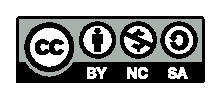
\includegraphics[width=3.0cm]{./img/static/Cc-by-nc-sa_icon.eps}}\par
\vspace*{3\baselineskip}
\endgroup}

\titleTH


%%% Local Variables:
%%% mode: latex
%%% TeX-engine: luatex
%%% TeX-master: "../retazosfisica.tex"
%%% End:



% -----------------------------------------------------------------------------
% Tabla de contenidos
\thispagestyle{empty}
% tablacontenidos.tex
% Tabla de contenidos.
%
% Copyright (C) 2025 José A. Navarro Ramón <janr.devel@gmail.com>
% Licencia Creative Commons Recognition Share alike.
% (CC-BY-SA)

\tableofcontents

%%% Local Variables:
%%% mode: latex
%%% TeX-engine: luatex
%%% TeX-master: "../retazosfisica.tex"
%%% End:

% -----------------------------------------------------------------------------
\frontmatter
% prologo.tex
%
% Copyright (C) 2025 José A. Navarro Ramón <janr.devel@gmail.com>
% Licencia Creative Commons Recognition Share-alike.
% (CC-BY-SA)

\chapter{Prólogo}



 
%%% Local Variables:
%%% mode: latex
%%% TeX-engine: luatex
%%% TeX-master: "../retazosfisica.tex"
%%% End:

% -----------------------------------------------------------------------------
% Teoría
\mainmatter
%\part{Teoría}
% mecanicaestadistica.tex
%
% Copyright (C) 2025 José A. Navarro Ramón <janr.devel@gmail.com>
% Licencia Creative Commons Recognition Share-alike.
% (CC-BY-SA)

\chapter{Mecánica estadística}
Este capítulo se desarrolla a nivel básico la mecánica estadística
de Maxwell-Boltzmann, la de Bose-Einstein y la de Planck.

\section{Estadística de Maxwell-Boltzmann}
Boltzmann fue un físico austriaco pionero de la mecánica estadística y se
encontró con la incomprensión de muchos físicos de su tiempo, pues el
atomismo no estaba del todo aceptado. Al poco de morir ---comienzos del siglo
XX--- se acumularon más evidencias a favor de los átomos, de modo que esta
quedó completamente aceptada poco después.
%[Wikipedia]

\subsection{Modelo teórico}
En este modelo, se considera un número $N$ enorme de partículas distinguibles
de cualquier spin y que están lo suficientemente separadas entre ellas como
para que la única interacción entre ellas sea la colisión elástica entre ellas,
por tanto, se desprecia la interacción a distancia entre ellas, esto es,
energía potencial de cualquier tipo, eléctrica o gravitatoria.
% [Arthur Beiser]

Un ejemplo típico al que se le puede aplicar el modelo es el de un gas formado
por moléculas ---átomos o grupos de átomos neutros---.

Las $N$ partículas, $n_1, n_2, \cdots, n_k$, se distribuyen entre $k$ estados
de energía creciente,  $u_1, u_2, \cdots, u_k$ . Estos estados pueden ser,
bien estados discretos o energías medias de una secuencia creciente de
intervalos continuos. Incluso, como el modelo es clásico, el número de niveles
$k$ puede ser muy elevado, y se podría considerar que estas forman un
continuo (esto lo utilizaremos posteriormente).









%%% Local Variables:
%%% mode: latex
%%% TeX-engine: luatex
%%% TeX-master: "../retazosfisica.tex"
%%% End:

% matrizdensidad.tex
%
% Copyright (C) 2020-2025 José A. Navarro Ramón <janr.devel@gmail.com>
% 1) Código fuente:
% Licencia GNU-2
%
% 2) Texto legible en cualquier formato: pdf, postscript, html, etc.:
% Licencia Creative Commons Recognition-NonCommercial-ShareAlike.
% (CC-BY-NC-SA)
% ----------------------------------------------------------------------------

\chapter{Matriz Densidad}

\section{Operador densidad}
Vamos a utilizar un espacio de Hilbert $\left(\mathbb{C}^2\right)$, de
dimensión 2, por comodidad
\[
  \mathlarger{\mathcal{H} = \mathbb{C}^2}
\]

Lo siguiente es elegir los símbolos de una base. Se podrían elegir algunos
símbolos como $\ket{\varphi_1}$ y $\ket{\varphi_2}$, $\ket{e_1}$ y $\ket{e_2}$,
$\ket{a}$ y $\ket{b}$, etc. Pero vamos a introducir una nomenclatura que es
propia de la información cuántica y que hace referencia al \emph{qbit}.
De esta forma, la base\footnotemark{} la representaríamos como
\footnotetext{La base está formada por dos vectores en un espacio de Hilbert
  de dimensión 2. En general, tendría $n$ vectores.}
\[
  B = \{\ket{0}, \ket{1}\}
\]

El cero y el uno son solo etiquetas. No hay nada profundo en eso, solo inspiran
al bit clásico. Únicamente decir, por completitud, que por \emph{qbit} se
entiende aquel vector que es una combinación lineal de estos dos vectores de la
base
\[
  \bra{\Psi} = a \ket{0} + b \ket{1}
\]
pero no vamos a entrar en esto. Dejamos los \emph{qbits} a un lado.

A partir de ahora solo consideramos tener un espacio de Hilbert de dimensión 2
y estos dos vectores de la base.






%%% Local Variables:
%%% mode: latex
%%% TeX-engine: luatex
%%% TeX-master: "../retazosfisica.tex"
%%% End:

% -----------------------------------------------------------------------------
%% Apéndices
%%\backmatter
%%\part{Apéndices}
%\appendix
%\renewcommand{\thechapter}{A}
%\clearpage
%\addappheadtotoc
%\appendixpage
%%\include{./apendices/gl-momangcuantico-genfunciones}
% -----------------------------------------------------------------------------

\end{document}


%%% Local Variables:
%%% coding: utf-8
%%% mode: latex
%%% TeX-engine: luatex
%%% TeX-master: t
%%% End:
